\documentclass[a4paper,doc,floatsintext,natbib]{apa6}
% \documentclass{article, a4paper}
\usepackage[font=small]{caption}
\usepackage{lscape}
\usepackage{graphicx}
\usepackage{amsmath}
\usepackage{authblk}
\usepackage[utf8]{inputenc}
\usepackage{nameref}
\usepackage{hyperref}
\usepackage{cleveref}
\usepackage{soul}
\usepackage{todonotes}

% Remember to start reftex-mode

\hypersetup{
  colorlinks=true,
  linkcolor=black,
  citecolor=black,
  urlcolor=black
  }

\setlength{\parskip}{1em}
\def \fref #1{Figure \ref{#1}}     % Reference figures
\def \tref #1{Table \ref{#1}}      % Reference tables
\def \eref #1{Equation \ref{#1}}   % Reference equations
\def \sref #1{Section '\nameref{#1}'}    % Reference sections
\def \supmat {the Supplementary Materials}

\DeclareMathOperator*{\argmin}{argmin}
\DeclareMathOperator*{\argmax}{argmax}

% For revision
\DeclareRobustCommand{\newcontent}[1]{#1}

\title{The effects of context inference on motor learning: savings, de-adaptation and spontaneous recovery}
\shorttitle{Context-inference-dependent motor learning}
\author[1]{Cuevas Rivera, Darío}
\author[1]{Kiebel, Stefan J.}
\affil[1]{Chair of Neuroimaging, Faculty of Psychology. Technische Universität Dresden, 01062 Dresden, Germany.}
\affiliation{~}

\begin{document}

\maketitle

\abstract{Abstract}
% \tableofcontents

\section{Introduction}
yeah

\section{Results}
In this work, we present a motor adaptation model in which the agent (e.g. a human learning a motor task) updates an existing model of the environment based on error signals produced by the need of adaptation. Several models exist for error-based motor adaptation, but we expand on the existing models by adding an explicit component of context inference which guides the selection of the adequate internal model, its updating and the sampling of actions.

In what follows, we introduce the different parts of the model and explain how they work together. In addition, we will highlight experimental findings in motor adaptation from previous works for which our model provides explanations that are otherwise unavailable.

\subsection{The model}
The model we present has three main components: (1) a context-inference component; (2) a motor adaptation component; (3) an action selection component. Each of these components informs the ones that follow: motor adaptation is informed by context inference, and action selection is informed directly by both motor adaptation and by context inference.

Based on the Bayesian brain hypothesis, we chose to cast both context inference and motor adaptation as Bayesian inference, in effect using a unified mechanism for the preparation of motor commands in new environments.

We now describe the three components of the model separately. We begin by describing the motor adaptation part for clarity, as the definition of ``context'' (used in context inference) is better described in terms of motor adaptation.

\subsubsection{Motor adaptation}
Motor adaptation refers to the ability of humans and other animals to learn from observed errors. For example, we can learn to perform a reaching movement in front of us --a movement that any person has been practicing all their lives-- underwater, where the relatively high viscosity of water means that the motor commands we have learned all our lives no longer produce the desired effect.

It is widely accepted that in order to adapt motor commands to a novel environment, we create and update internal forward models of the outcomes of control signals. While a number of models for motor adaptation exist, we chose to make use of an exact Bayesian learner. As we discuss below, a Bayesian learner has the advantage of not only fitting experimental data on motor adaptation, but also does away with the need for explicit multiple time scales of learning. We show that this adaptation mechanism can deal with adaptation after any number of trials, ranging from a handful of trials in an experiment to the level of expertise a professional dancer has accrued through years of practicing the same movements.

To describe this component of the model, let us return to reaching movements. Throughout our lives, we have learned the equivalence between a motor command and its outcomes in the form of a forward model. We can write this forward model as follows:
\begin{equation}
p(\vartheta | s, c) = f(s, c; \beta)
\end{equation}
where $\vartheta$ are the outcomes of an action (in the example, direction and velocity of the reach movement), $s$ is the current state (e.g. the current position of the hand), $c$ is a motor command and $\beta$ are the parameters of the forward model $f(\cdot)$. Throughout our lives, the parameters $\beta$ have been fine tuned to produce an accurate forward model $f$ to guide our movements.

As a day progresses, and especially if the day included a lot of physical activity of the arm, muscle exhaustion leads to a different response of the muscles in the arm to motor commands. However, we are still able to produce accurate reach movements. This happens through adaptation, where the observed error signals of a moment are used to temporarily update the parameters $\beta$ of the forward model. To describe this adaptation process, our model makes uses of Bayesian inference, such that:
\begin{equation}
q(\beta | \vartheta, s, c) \propto p(\vartheta | s, c, \beta)p(\beta)
\end{equation}
where $q(\beta | ...)$ represents the new estimate of $\beta$ after having observed the outcome $\vartheta$ of the previous motor command $c$. $p(\vartheta | s, c, \beta)$ is the \textit{a priori} probability of observing the outcome $\vartheta$ as predicted by the forward model $f$, and $p(\beta$ is the previous estimate of $\beta$.

In this account of motor adaptation, the prediction error signal takes the form of an observed outcome $\vartheta$ that differs from that of the most likely outcome predicted by the forward model. The amount of adaptation that happens after observing an error will depend not only on the size of the error (how far away from the most likely outcome) it is, but also of how precise the existing estimate of $\beta$ is. We will discuss this further below.

Not only is the internal model for everyday movements not fixed (i.e. adaptation is possible), it is also not unique. Multiple internal models are used and updated, depending on the task at hand. For example, a person might have an internal model for baseline reaching movements (e.g. with empty hands) $f_B$, and a different one for reaching movements while holding a heavy object, $f_H$. A key aspect of motor adaptation is to select the relevant model to update, should a prediction error arise.

\subsection{Context inference}
In our model, the idea of context is quite general. The context comprises the relevant elements of hte environment (e.g. high winds when walking), as well as the task at hand. Previous models have focused on the elements of the context which are directly related to the internal models: given a past action, the different internal models (e.g. $f_B$ and $f_H$ from the previous section) make different predictions for the outcome of that action; the model that best predicts that action is deemed to be the ``correct'' model, i.e. the model that best represents the context.

In this work, we focus on the idea that the context can be inferred by integrating several sources of information, an idea with great intuitive appeal. Through this idea, we explain many previously-unexplained phenomena from different experiments with humans.

Identifying any possible context with a categorical variable $\zeta$, the identification of a context can be done through Bayesian inference:
\begin{equation}
q(\zeta | \vartheta_t, \vartheta_{t-1}, c_{t-1}) \propto p(\vartheta_t | \vartheta_{t-1}, c_{t-1})p(\zeta)
\end{equation}
where the prior distribution over contexts $p(\zeta)$ includes information from two sources: (1) an expectation of continuity, encoding the expectation that the context does not change from instant to instant, and (2) an overall estimation of observing any one context, if the context did change. Below, we discuss how these two components effect different experimentally observed phenomena.

In the previous section, we used the variable $\vartheta$ to refer to the outcomes of actions. In this section, we expand the definition of an observation $\vartheta$ to include any information given to the decision-making agent by the environment. This includes, as before, the outcomes of actions, but also any other sensory information that might be indirectly related to actions, or even completely intependent from them. For this section, the most important component of $\vartheta$ is contextual information, i.e. information that might directly help infer the identity of the current context.

In experimental settings, the contextual information can take the form of a visual cue [EGS], the place where the task must be carried out [EGS] or even the start of a new block of trials [EGS]. All these sources of information, alongside the outcomes of previous actions and the priors $p(\vartheta$ form part of $p(\vartheta_t | \vartheta_{t-1
}, c_{t-1})$ and are integrated together to identify a context.

\subsection{Action selection}
Action selection is affected by the current context via the context-dependent forward model that is used. In our model, action selection is made by building a distribution over available actions which is a weighted sum of the distributions given by the existing forward models, where the weights are obtained by the context inference component of the model. In other words, a distribution is created as follows:
\begin{equation}
p(c_t) \propto \displaystyle\sum_{\zeta \in \Phi}q(\zeta | \vartheta_t, \vartheta_{t-1}, c_{t-1}) p(c_t | \zeta)
\end{equation}
From this distribution, the current action (motor command $c_t$) can be sampled and carried out.

\section{Experimental results}
In this section, we go through a number of experimentally-observed phenomena and show how imperfect context inference, as done in our model, provides a parsimonious explanation for all of them.

In what follows, we show numerical results obtained the model outlined above. The full mathematical implementation of the model can be found in \sref{subsection:model-description}.

Before discussing these phenomena, let us introduce terminology. As an example, we will use a typical motor adaptation task in which participants have to make forward-backward reaching movements while holding the handle of a mechanical arm that exerts a force. Depending on the trial (and experiment), the arm might exert a curl force in a clockwise or counter-clockwise direction, or no force at all. Let us define the baseline context O as that in which the mechanical arm exerts no force. Context A can be defined as that in which the arm exerts the clockwise curl force and context B counter-clockwise. Additionally, abusing notation, it can be said that $B = (-A)$, as the forces point (approximately) in opposite directions. We represent contexts such as A and A/2, which means that both have the same direction of the adaptation (e.g. clockwise), but the second one has half the magnitude. Finally, we represent error-clamp trials with the letter E and washout trials with W.

With this terminology, a typical experiment [EGs] would have a block structure of O-A-B-E (or O-A-(-A)-E), which means that the participant goes through a block of trials with no external force applied (O), a number of trials with a clockwise curl force (A), a block with counter-clockwise forces (B), and finally a block with error-clamp trials (E).

\subsection{Savings and quick de-adaptation}
Savings refers to the ability of humans and other animals to remember a previously-learned adaptation and apply it without having to re-learn it. Savings is almost universally observed in human participants [A THOUSAND CITATIONS, c.f. papers with volatility or ramping up/down], but animal experiments have shown mixed results \citep[e.g.][]{Kojima_Memory_2004}. In an O-A-O-A experiment, for example, savings would be seen in the second A block in the form of an adaptation rate apparently higher than that observed during the first A block.

On the other hand, quick de-adaptation refers to the observation that in an O-A-O paradigm, the adaptation from O to A is much slower than that from A back to O.

In this section, we will show that both phenomena are the two sides of a coin, and the speed at which this quick adaptation/de-adaptation happens, which is known not to be immediate [Citations] is related to the availability and reliability of contextual information, as well as to the quality of the prediction errors.

To show this, we categorized experiments performed with human participants by looking at the amount of contextual information that is available. In some experiments [EGssss], the context is clearly \todo{Maybe not use the word 'cue', as many experiments don't have explicit sensory cues}cued to the participant, e.g. in the form of visual cues [EGs] or in changes to the location of the task [EGs]. We call these cued-context experiments. In other experiments, partial information is available to participants [EGsss]; we refer to these as partially-cued experiments. While there are no experiments in which no contextual information is available, there are some experiments which contain blocks of trials in which no contextual information is available and participants have no way of inferring the current context. Abusing our notation, we call these experiments (or rather, these sections of the experiments) uncued experiments. In this section, we focus on the two former categories, while the latter is left for the next sections.

Note that, because context inference integrates information from many sources, many experiments in which no intentional, overt contextual cues are available indeed contain contextual information that the participant can use. For example, in curl-force-field experiments with mechanical arms, the force feedback provided by the mechanical arm always gives participants a sense for the current context, although error-clamp trials are difficult to distinguish from adaptation trials based on force feedback alone. Proprioceptive signals can also provide contextual information [EGs of experiments with hidden hands]. The sudden appearance of motor errors can itself be a cue for contextual change, as long as the motor error is perceivably higher than normal trial-by-trial variation in performance.

In FIGURE XXX, we show data from representative experiments from the cued-context \citep{Kim_Neural_2015} and partially-cued \citep[][group 1c]{Oh_Minimizing_2019} categories are shown. \cite{Kim_Neural_2015} used a colored light as a visual cue at the beginning of each experiment, whereas \cite{Oh_Minimizing_2019} included a condition in which the necessary adaptation was in the order of the motor error, making feedback-based context inference slow. It can be seen that in cued-context experiments \cite[data from][]{Oh_Minimizing_2019}, savings take the form of an immediate switch from the adaptation at trial $t$ to that in trial $t-1$, to the level that was learned before. In contrast, in partially-cued experiments, the switch is fast (compared to the initial adaptation), but not immediate. Our model explains this difference via context inference: in the cued-context experiments, context inference relies on the very reliable information of visual cues and the change in context is identified immediately; because of this, the model can re-activate the forward model adequate for the context from the first trial after the change occured. In contrast, in partially-cued experiments, the model needs to accumulate evidence in favor of the correct context throughout a number of trials, and the actions selected by the model are combinations of the actions that correspond to all the possible contexts (we discuss this in the following sections).

\begin{figure}
\centering
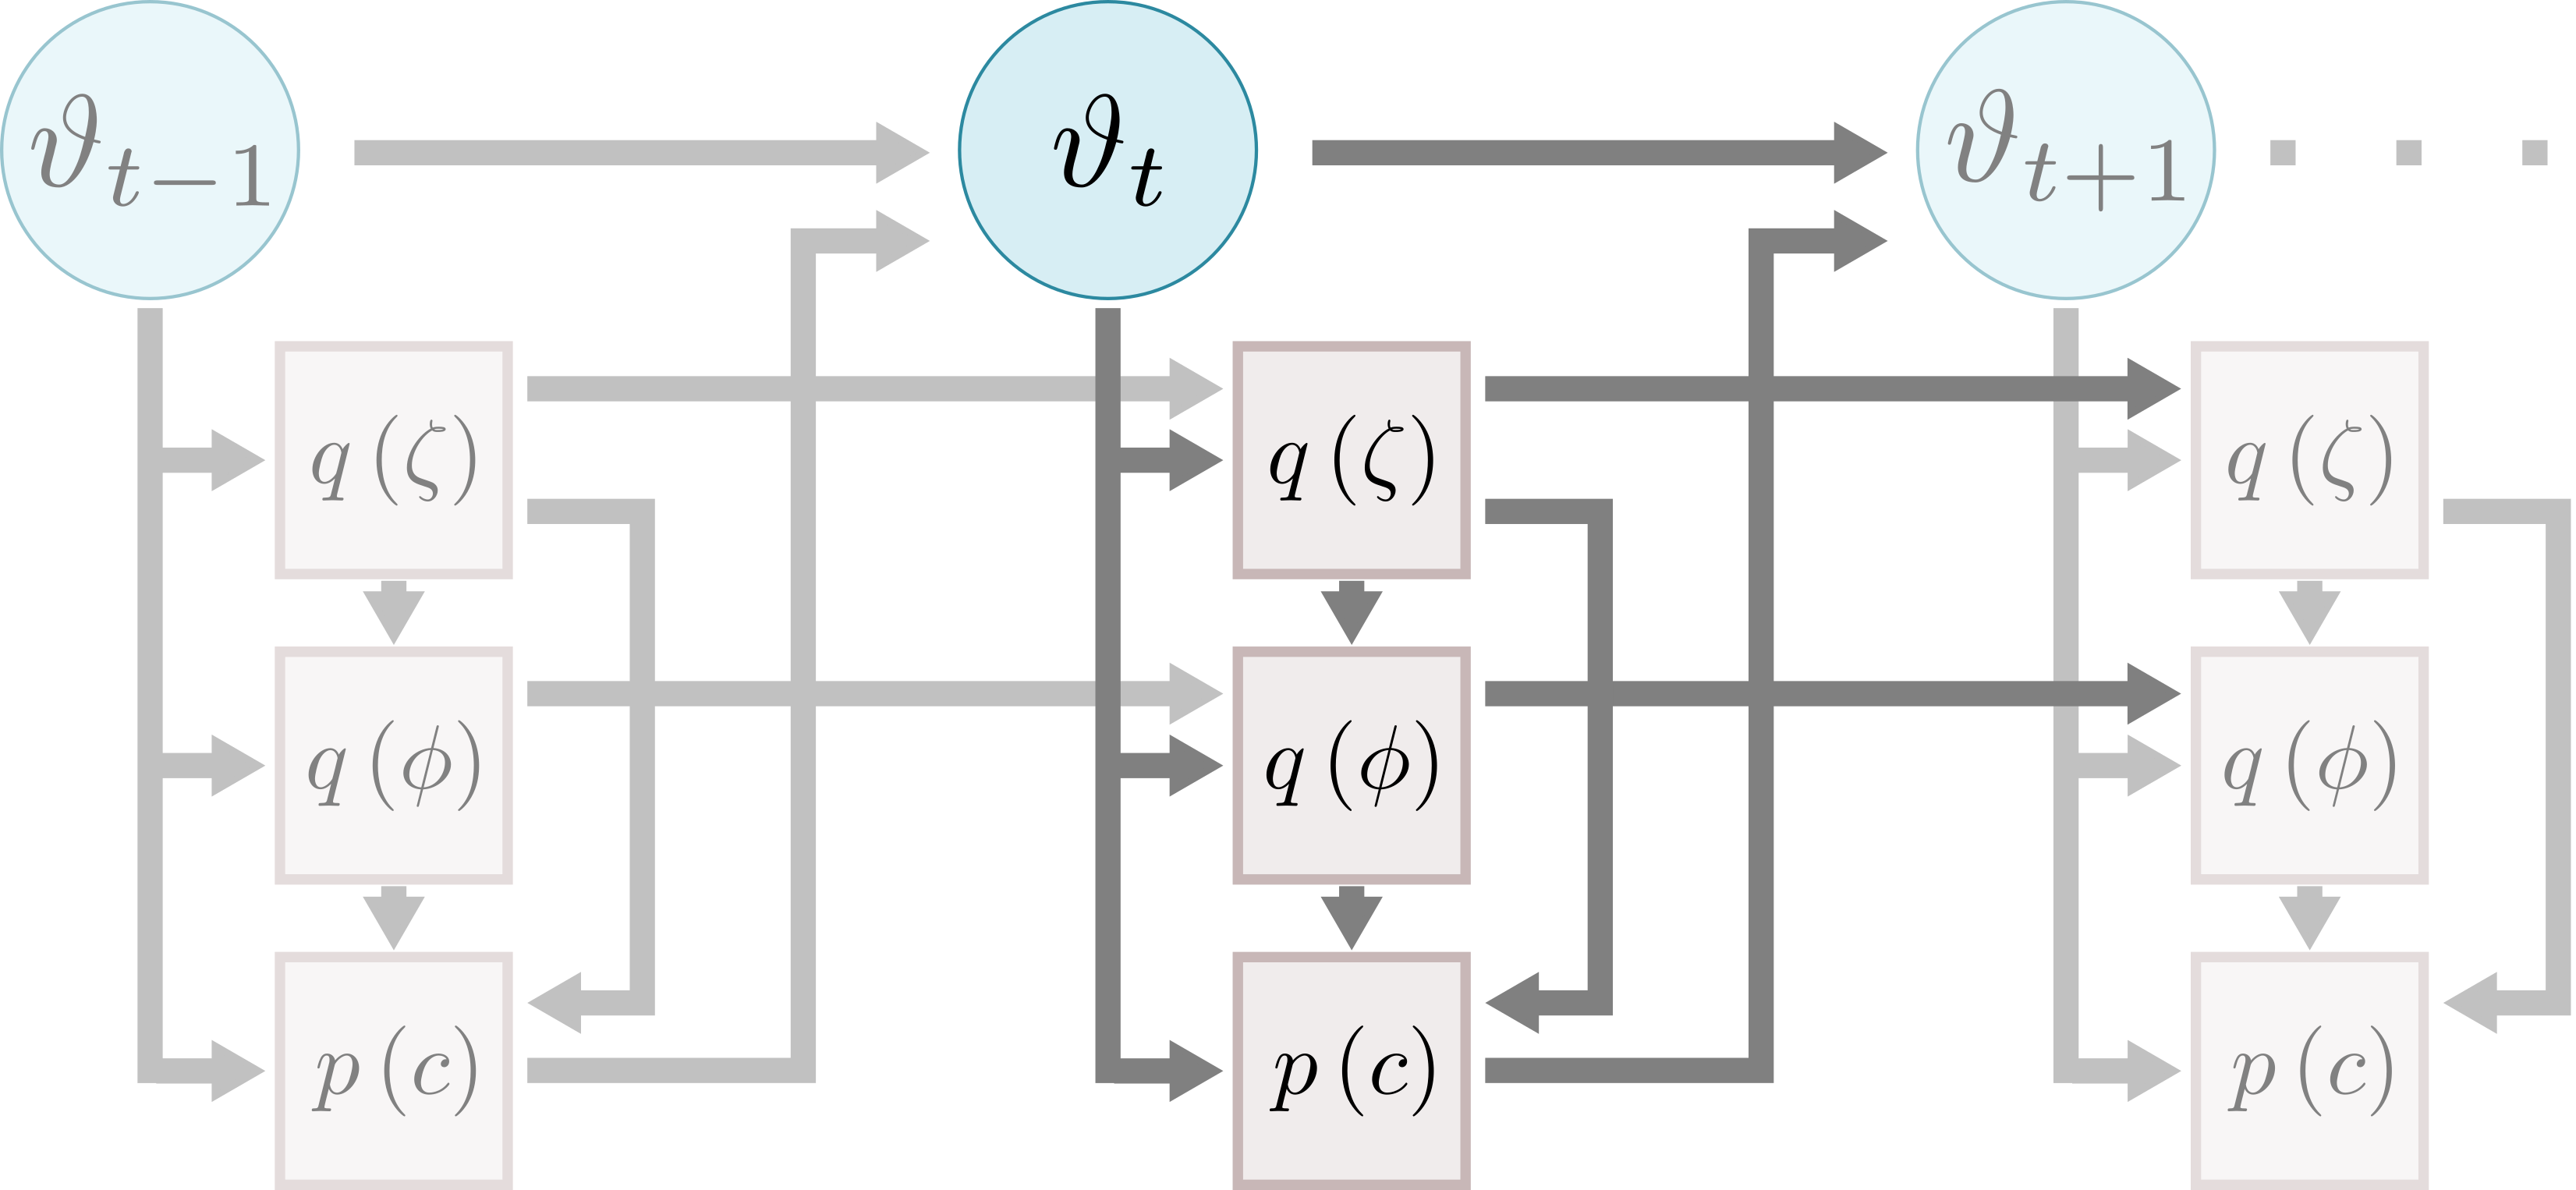
\includegraphics[width=\textwidth]{./figures/figure_1.png}
\caption{Savings and de-adaptation. Data from our simulations (A and C) compared to data from \cite{Oh_Minimizing_2019} (B and D). In all panels, the blue line represents the adaptation displayed by the agent as a function of trial number. The black lines represent the optimal adaptation, i.e. the size of the visuomotor rotation during the task. (A) A simulated experiment in which the agent must adapt to a 20 degree visuomotor rotation during shooting movements. It can be seen that after context switches (e.g. at trial 120), the agent returns to the adaptation of the previous block, with one or two trials of delay. (B) Data adapted from \cite{Oh_Minimizing_2019}, figure 4a. The same immediate switch can be observed as that in A. (C) Simulated experiment with a 10 degree adaptation. In this case, savings are much slower. (D) Data adapted from \cite{Oh_Minimizing_2019}, figure 4a.} \label{fig:oh-2019}
\end{figure}

Note that in the data from \cite{Oh_Minimizing_2019} and \cite{Kim_Neural_2015} include both savings (O-A transitions) and de-adaptation (A-O transitions), both of which display the same characteristics and are explained by the same mechanism in our model. \todo{Need to be careful here, as de-adaptation is sometimes discussed only in terms of experiments with no contextual cues or where the meaning of the cues is inverted}.


\section{The effects on the rate of adaptation}
In our model, adaptation is gated by the uncertainty on the current context. More specifically, a prediction error observed at trial $t$ will effect motor adaptation with a magnitude proportional to the size of the error, where the proportionality constant is related to the uncertainty over the context in which the error was observed: the higher the uncertainty, the lower the size of the adaptation, given a fixed size of prediction error.

The most direct evidence for the effects of context inference on the rate of adaptation come from the experiments by \cite{Herzfeld_memory_2014}. The authors showed that the volatility of the environment, expressed in terms of unpredictable, stochastic transitions between A and -A (and vice versa) change the speed at which adaptation occurs.

\cite{Herzfeld_memory_2014} used an experimental paradigm in which the force that a mechanical arm exerts on the participant's hand can change from trial to trial between two possibilities: no force (baseline O) a clockwise force (context A) and a counter-clockwise force (context -A). They divided participants into three groups for which the transition from one trial to the next were very uncommon, somewhat common and almost every trial. Importantly, these transitions were uncued, and the participant could only infer that a transition had occurred after a motor error was observed.

\cite{Herzfeld_memory_2014} found that the volatility of the environment affects learning. The more volatile the environment, the less participants adapt their motor responses after observing an error. In \fref{fig:herzfeld-2014}, we show results obtained with our model in a paradigm matching that of \cite{Herzfeld_memory_2014}. We simulated the conditions of low volatility and maximum uncertainty ($z = 0.9$ and $z = 0.5$ in \cite{Herzfeld_memory_2014}) for thirty trials, repeating the experiment 300 times with random sequences of A and -A each time, following the transition probabilities from the experiment. In \fref{fig:herzfeld-2014}A we show the adaptation as a function of trial number, averaged across all 300 runs. It can be seen that the agent learns more slowly on the more volatile environment ($z = 0.5$) than on the less volatile one, matching the results from \cite{Herzfeld_memory_2014}. Additionally, \fref{fig:herzfeld-2014}B shows the sensitivity to errors, here defined as $\text{adaptation} / \text{error}$; the more volatile environment creates a lower sensitivity to errors than the predictable environment.

\begin{figure}
\centering
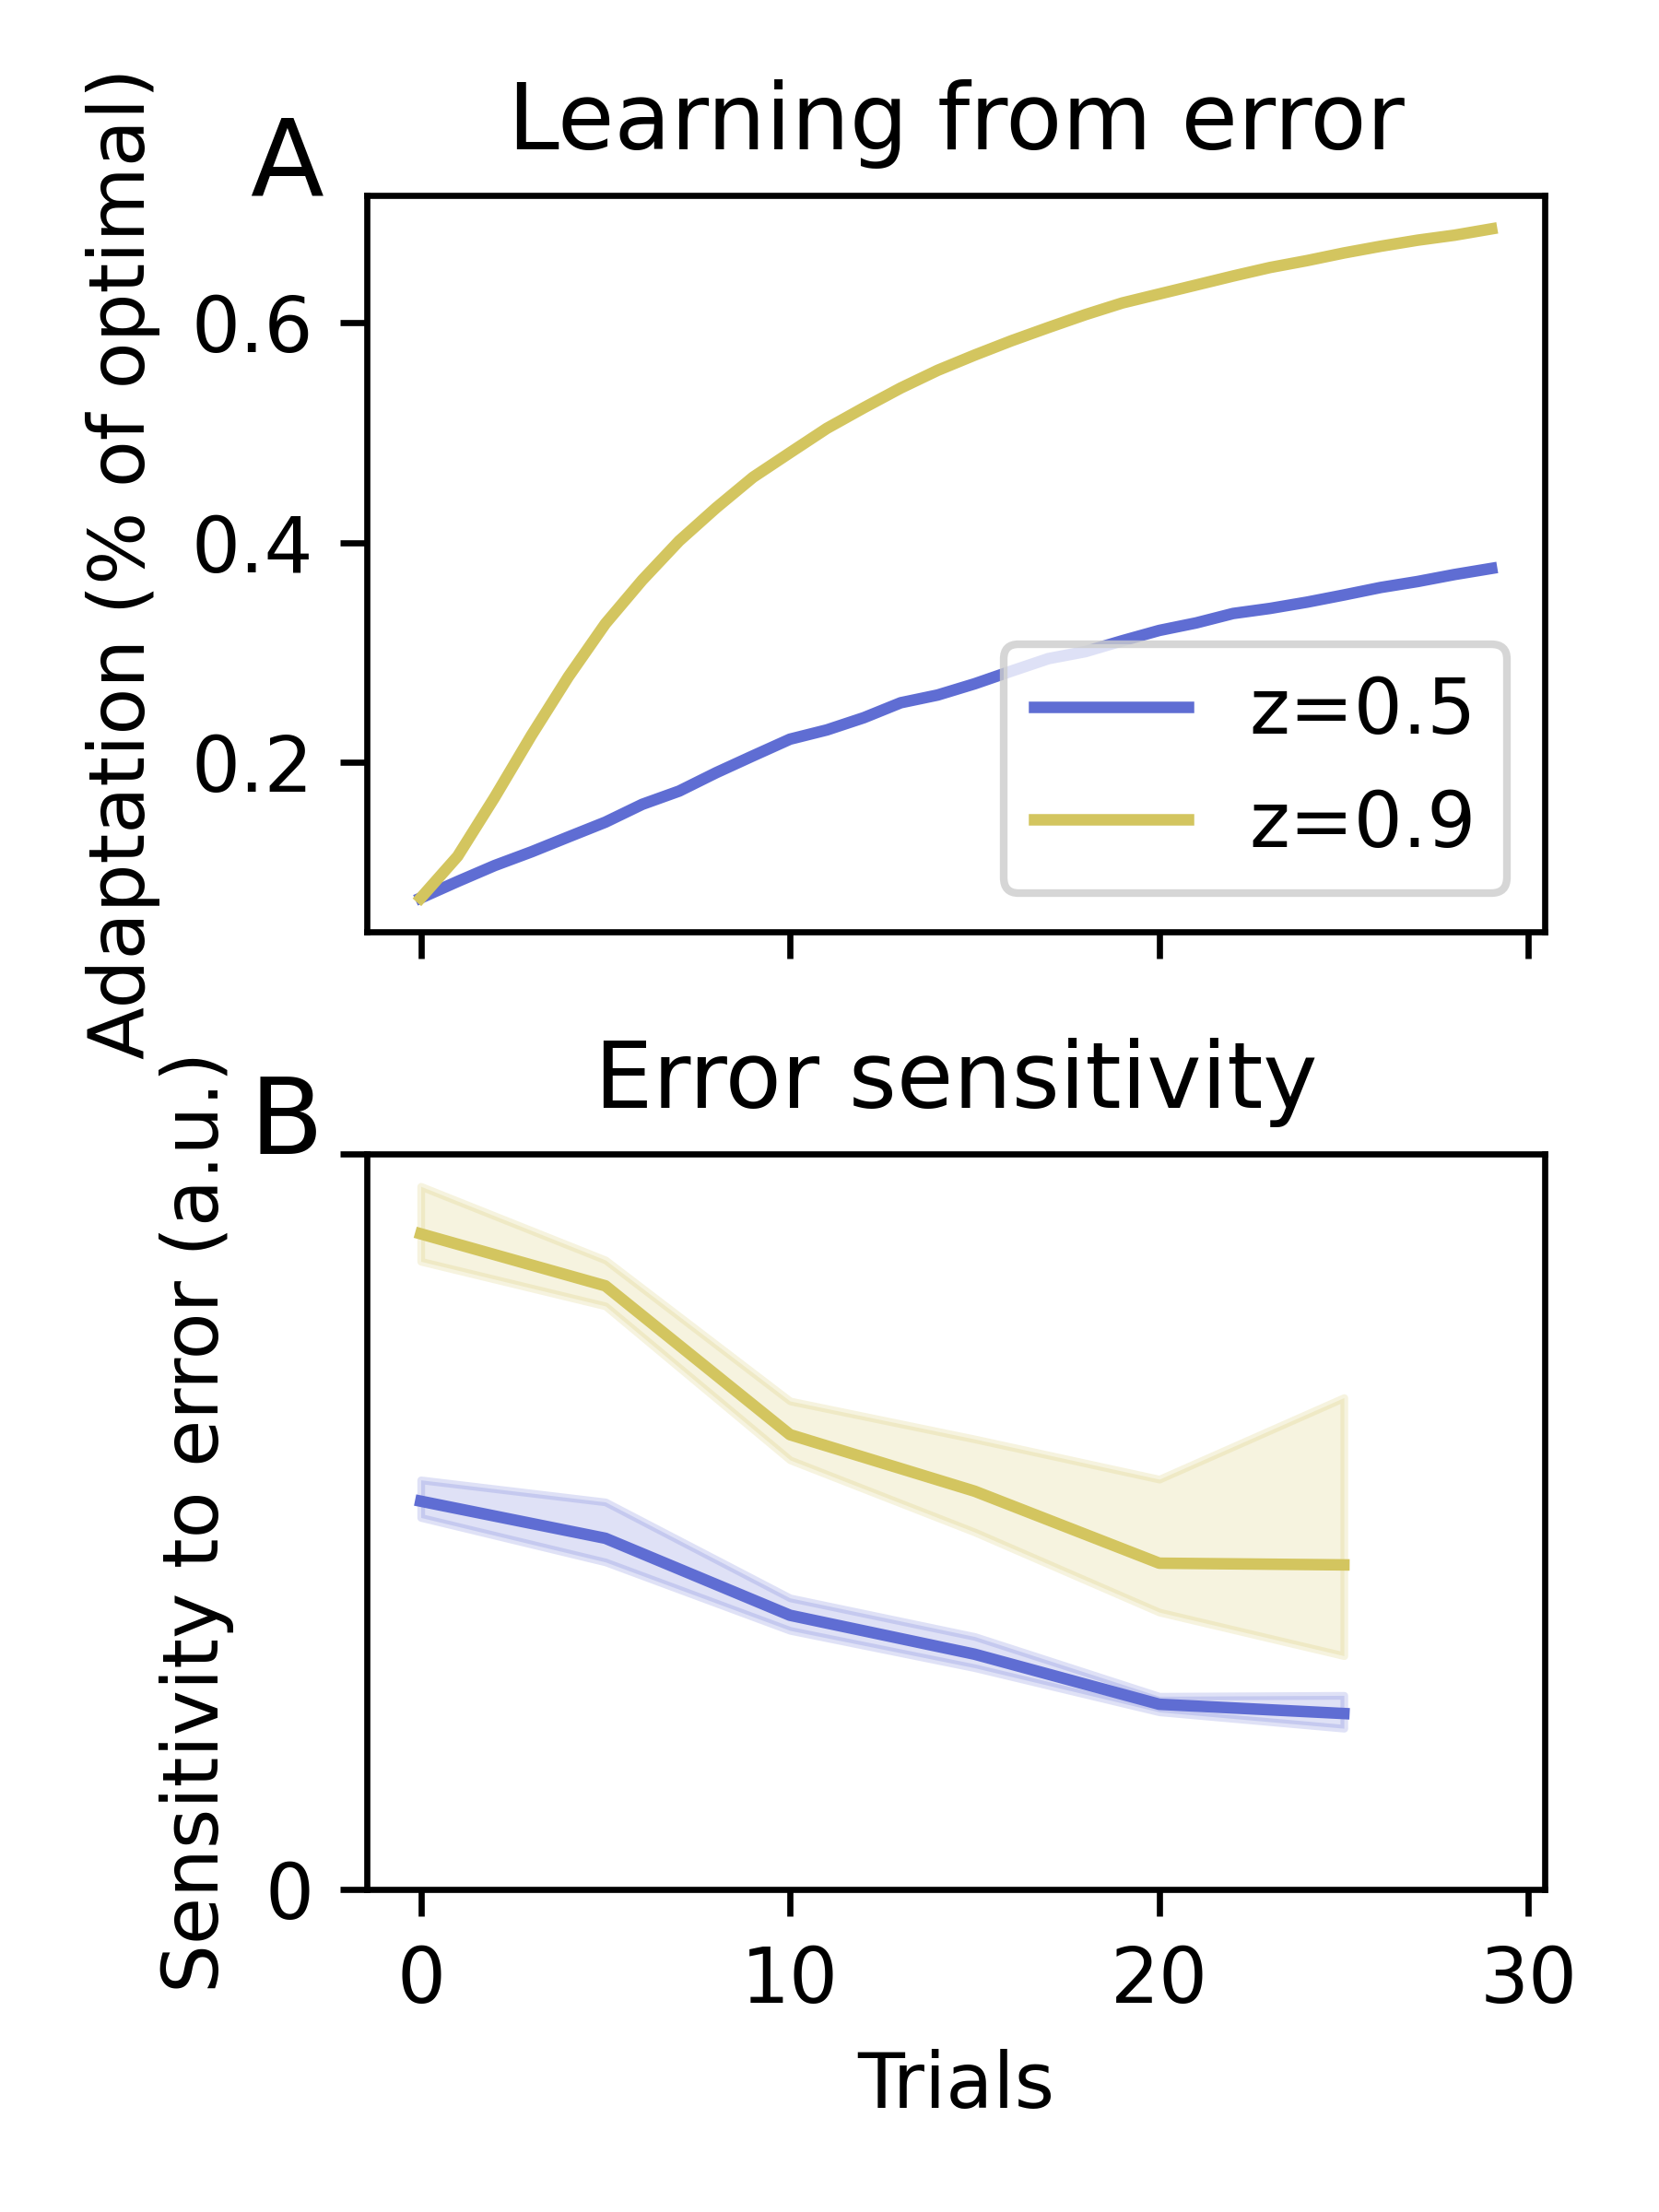
\includegraphics{./figures/figure_2.png}
\caption{Learning under unstable and unpredictable contexts. 30 trials were simulated in the task defined by \cite{Herzfeld_memory_2014}, repeated 300 times for better statistics. Two conditions were used, following the naming convention from \cite{Herzfeld_memory_2014}: $z=0.5$ is an unpredictable condition, where the context has a 0.5 probability of switching from trial to trial. $z=0.9$ is a stable condition, where the context has a 0.9 probability of staying the same from trial to trial. (A) Adaptation as a function of trial number, averaged across all runs. (B) Error sensitivity, binned into bins of 5 trials, averaged across all runs. The error is in arbitrary units, causing sensitivity to error (y axis) to also be in arbitrary units. Shaded areas are SEM.}
\label{fig:herzfeld-2014}
\end{figure}

In our model, learning is gated by context inference: the higher the uncertainty on the context in which an error occured, the lower the effect of this error on future trials (i.e. adaptation).

To account for volatility, the model includes a term in context inference which assumes a transition from the previous context to all other possible contexts (see Methods). Effectively, this transition term gives the model uncertainty on the current context, regardless of observations. The higher the volatility, the higher the uncertainty.

\section{Action selection}
As with learning, our model selects actions (motor commands) based on context inference. If the identity of the current context is known, the forward model for this context is used to select the current action. However, if some uncertainty exists, the selected action is influenced by all the possible current contexts, with a weight directly related to how likely each one of those contexts is.

Experimental evidence supporting this view can be found in experiments with context switching. For example, \cite{Davidson_Scaling_2004} reported an experiment in which participants had to switch from 3A to A in one group, with a block sequence A-3A-A-3A, and from -A to A in another group (where -A refers to an adaptation in the opposite direction as A, but with the same magnitude), with a block sequence A-(-A)-A-(-A), keeping the size of the necessary adaptation equal across both groups. After A and 3A in one group, A and -A in the other, had been learned in the first two blocks, the authors found that the switch from 3A to A was faster than that from -A to A. The authors interpreted this as evidence that a new adaptation happens more quickly if it is in the same direction as the current adaptation (e.g. both counter-clockwise), and more slowly if they are in the opposite direction (e.g. clockwise to counter-clockwise).

Our model offers a different explanation for the observed results: the assymetry is due to the existance of the baseline context. As discussed above, action selection in our model is done via a weighted avarage:
\begin{equation}
p(a_t | s_t) \propto \displaystyle \sum_{m \in M} p(m | s_t, s_{t-1}, a_{t-1}) p(a_t | m)
\end{equation}
In experiments without cued contexts, the baseline model $m_O$ has a non-zero probability $p(m | s_t ...)$. When a new block of trials starts (e.g. in the transition from 3A to A), a switch is inferred by the model (given feedback after the first trial) and $m_O$ becomes more likely (given that $m_{3A}$ has been ruled out. Therefore, in these first trials, action selection has a component guided by the baseline model, in which no extra compensatory force is applied, essentially ``pulling'' adaptation towards zero (no compensatory force). In the first group, this initial pull towards zero accelerates the transition towards A, as $3A > A > 0$, but on the second group, it slows down the switch because $A > 0 > -A$.

We simulated data with our model fitting the experimental structure by \cite{Davidson_Scaling_2004}. We show the results in \fref{fig:davidson-2004}, alongside the experimental results from \cite{Davidson_Scaling_2004}. It can be seen that the agent exposed to the -8 context shifts back to 4 more slowly than the one exposed to +8, qualitatively reproducing the data from \cite{Davidson_Scaling_2004}, shown in \fref{fig:davidson-2004}B.

\begin{figure}
\centering
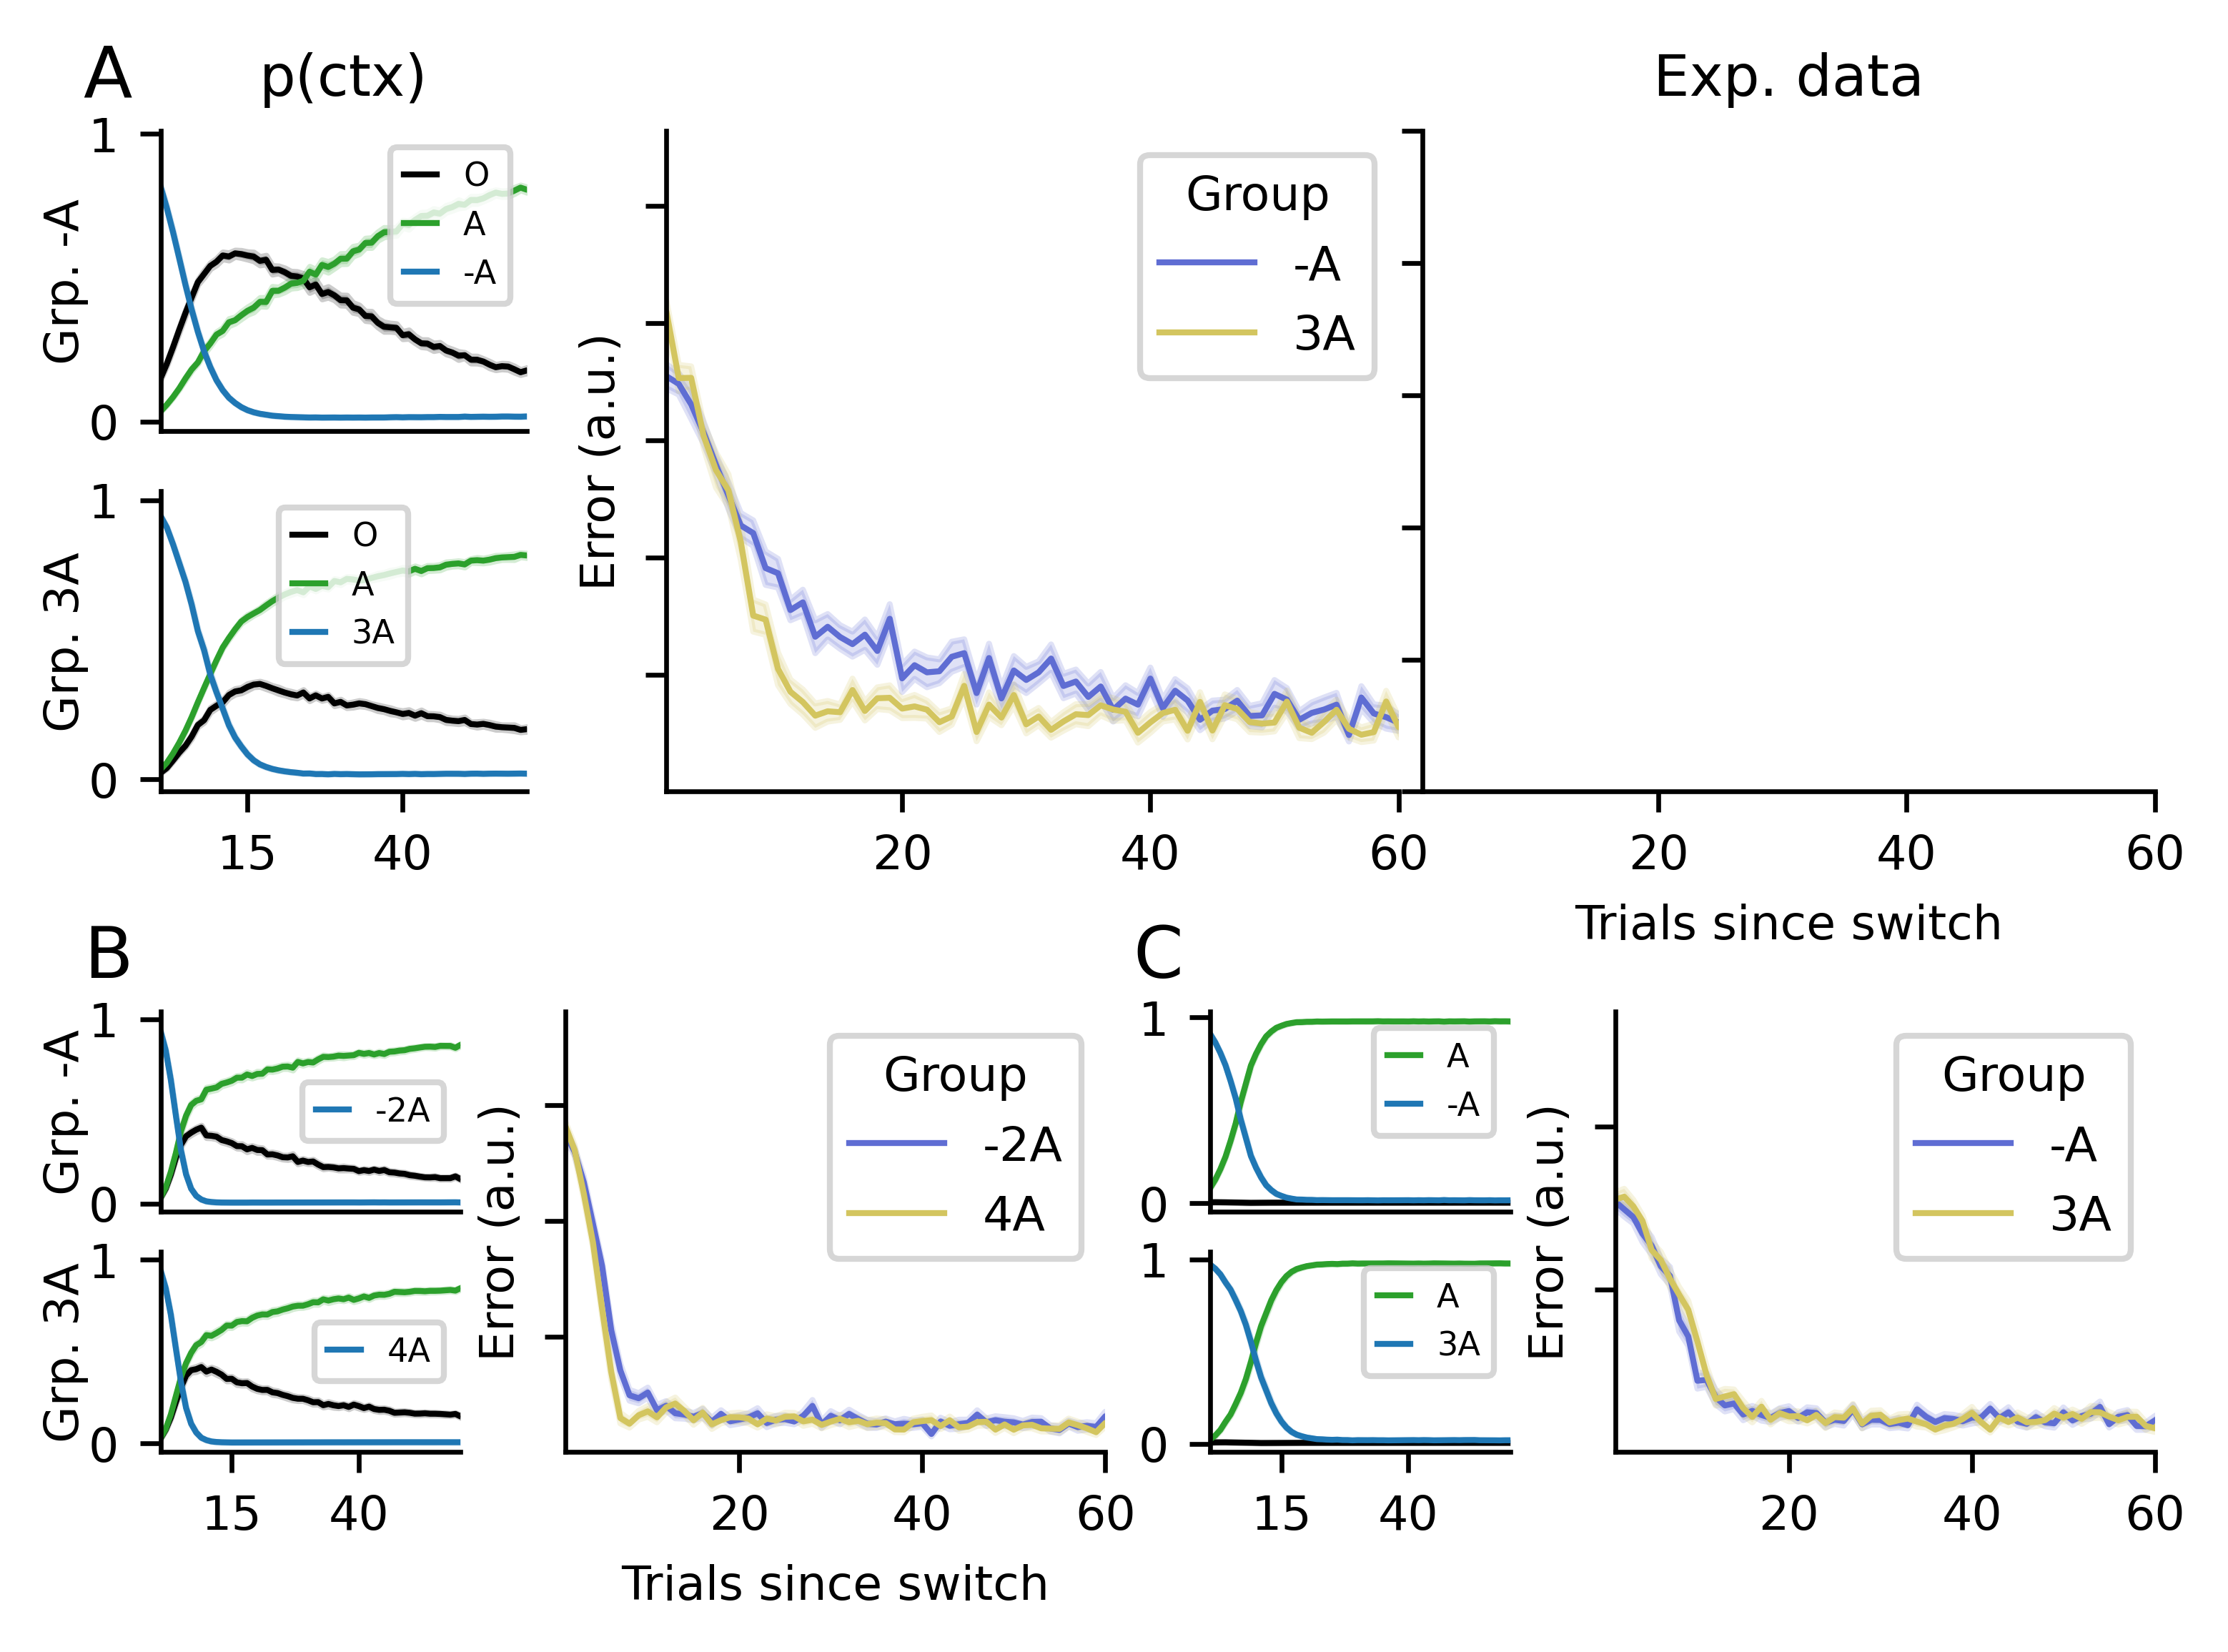
\includegraphics[width=\textwidth]{./figures/figure_3.png}
\caption{Motor error when switching back to a previously learned adaptation. Following the block structure from \cite{Davidson_Scaling_2004}, the first 40 trials of the switch from +8 (yellow) or -8 (blue) to 4 is shown. (A) Simulations from our model, with the task parameters from \cite{Davidson_Scaling_2004}. On the y axis, the error is shown in arbitrary units, related to centimiters through a monotonically increasing transformation with the same origin. (B) Data adapted from \cite{Davidson_Scaling_2004}, showing the error in the same trials as (A).}
\label{fig:davidson-2004}
\end{figure}

The model additionally predicts that the difference in observed switching speed between 3A-A and (-A)-A would disappear in an experiment in which the adaptations do not cross the baseline, i.e. all are positive or all are negative, or in an experiments in which the contexts are clearly cued. \todo{Maybe add simulations that show this, as well as simulations where the baseline context is not present.}

Further evidence can be found during error-clamp blocks in several experiments. We discuss these experiments in the following section. Additionally, we discuss experiments similar to that by \cite{Davidson_Scaling_2004} in the Discussion section.


\subsection{Action selection in error-clamp blocks}
During error-clamp blocks at the end of block sequences, participants' behavior can be described as the display of spontaneous recovery during the early trials of the E block, followed by a slow return to baseline across as many as hundreds of trials. However, the direction of the spontaneous recovery, its length, the delay before it is observed, the speed of the return to baseline and the final asymptote of the adaptation seem to vary greatly depending on the experiment.

In this section, we show how our model can explain these different parameters of behavior by changing the way contextual cues mislead participants' context inference, which in turn influences action selection.

\cite{Vaswani_Decay_2013} explored in detail human behavior during an error-clamp block in a shooting movement paradigm with a mechanical arm. The authors found that during an E block at the end of each experiment, there was a lag of a few trials (depending on participant) before their motor behavior changed from that of the previous trial. After that, the exerted force slowly dropped towards zero throughout tens of trials, but never reaching values around zero. Participants were divided into four groups, each of which going through a different block sequence: (1) A-E, (2) O-A-E, (3) (-A/2)-A-E, and (4) (-A)-E. No pauses were made during the experiment nor were there any contextual cues, so transitions between blocks were not signaled to participants. However, the mechanical arm used in the experiment provided force-feedback to participants.

In \fref{fig:vaswani-2013}A-E, we show the data simulated with our model for the task presented by \cite{Vaswani_Decay_2013}. The motor adaptation periods can be observed in \fref{fig:vaswani-2013}A-D for the four groups in the experiment, while on each bottom panel the inference over context is shown. Context inference works reliably until the error-clamp trials start, which do not correspond to any of the known contexts. This causes the agent to infer the combination of some of the known contexts that best fits the observations. Depending on the contexts learned by the agent (which change from group to group), inference during E trials will vary: groups 1.1 and 1.3 have exactly the same behavior, where the previous context (A and -A, respectively) slowly dwindles. These agents will slowly lower the force applied until eventually reaching zero (after hundreds of trials; not shown). In contrast, group 1.3 has the additional -A/2 context (represented by brown in \fref{fig:vaswani-2013}C, which has a non-zero posterior probility during E trials, pushing the agent's adaptation force more quickly towards zero. Group 1.2 behaves similarly to 1.1, with the exception that the baseline context, which was recently seen, plays a bigger role during E trials, making the agent reduce its force during E trials slightly more slowly than groups 1.1 and 1.4.

In \fref{fig:vaswani-2013}E, the same data is shown but only in the E trials. Here, the difference in the speed in which the force decays for the different groups is more readily visible. This is a strong qualitative match to the data from \cite{Vaswani_Decay_2013}, shown in \fref{fig:vaswani-2013}F.

\begin{figure}
\centering
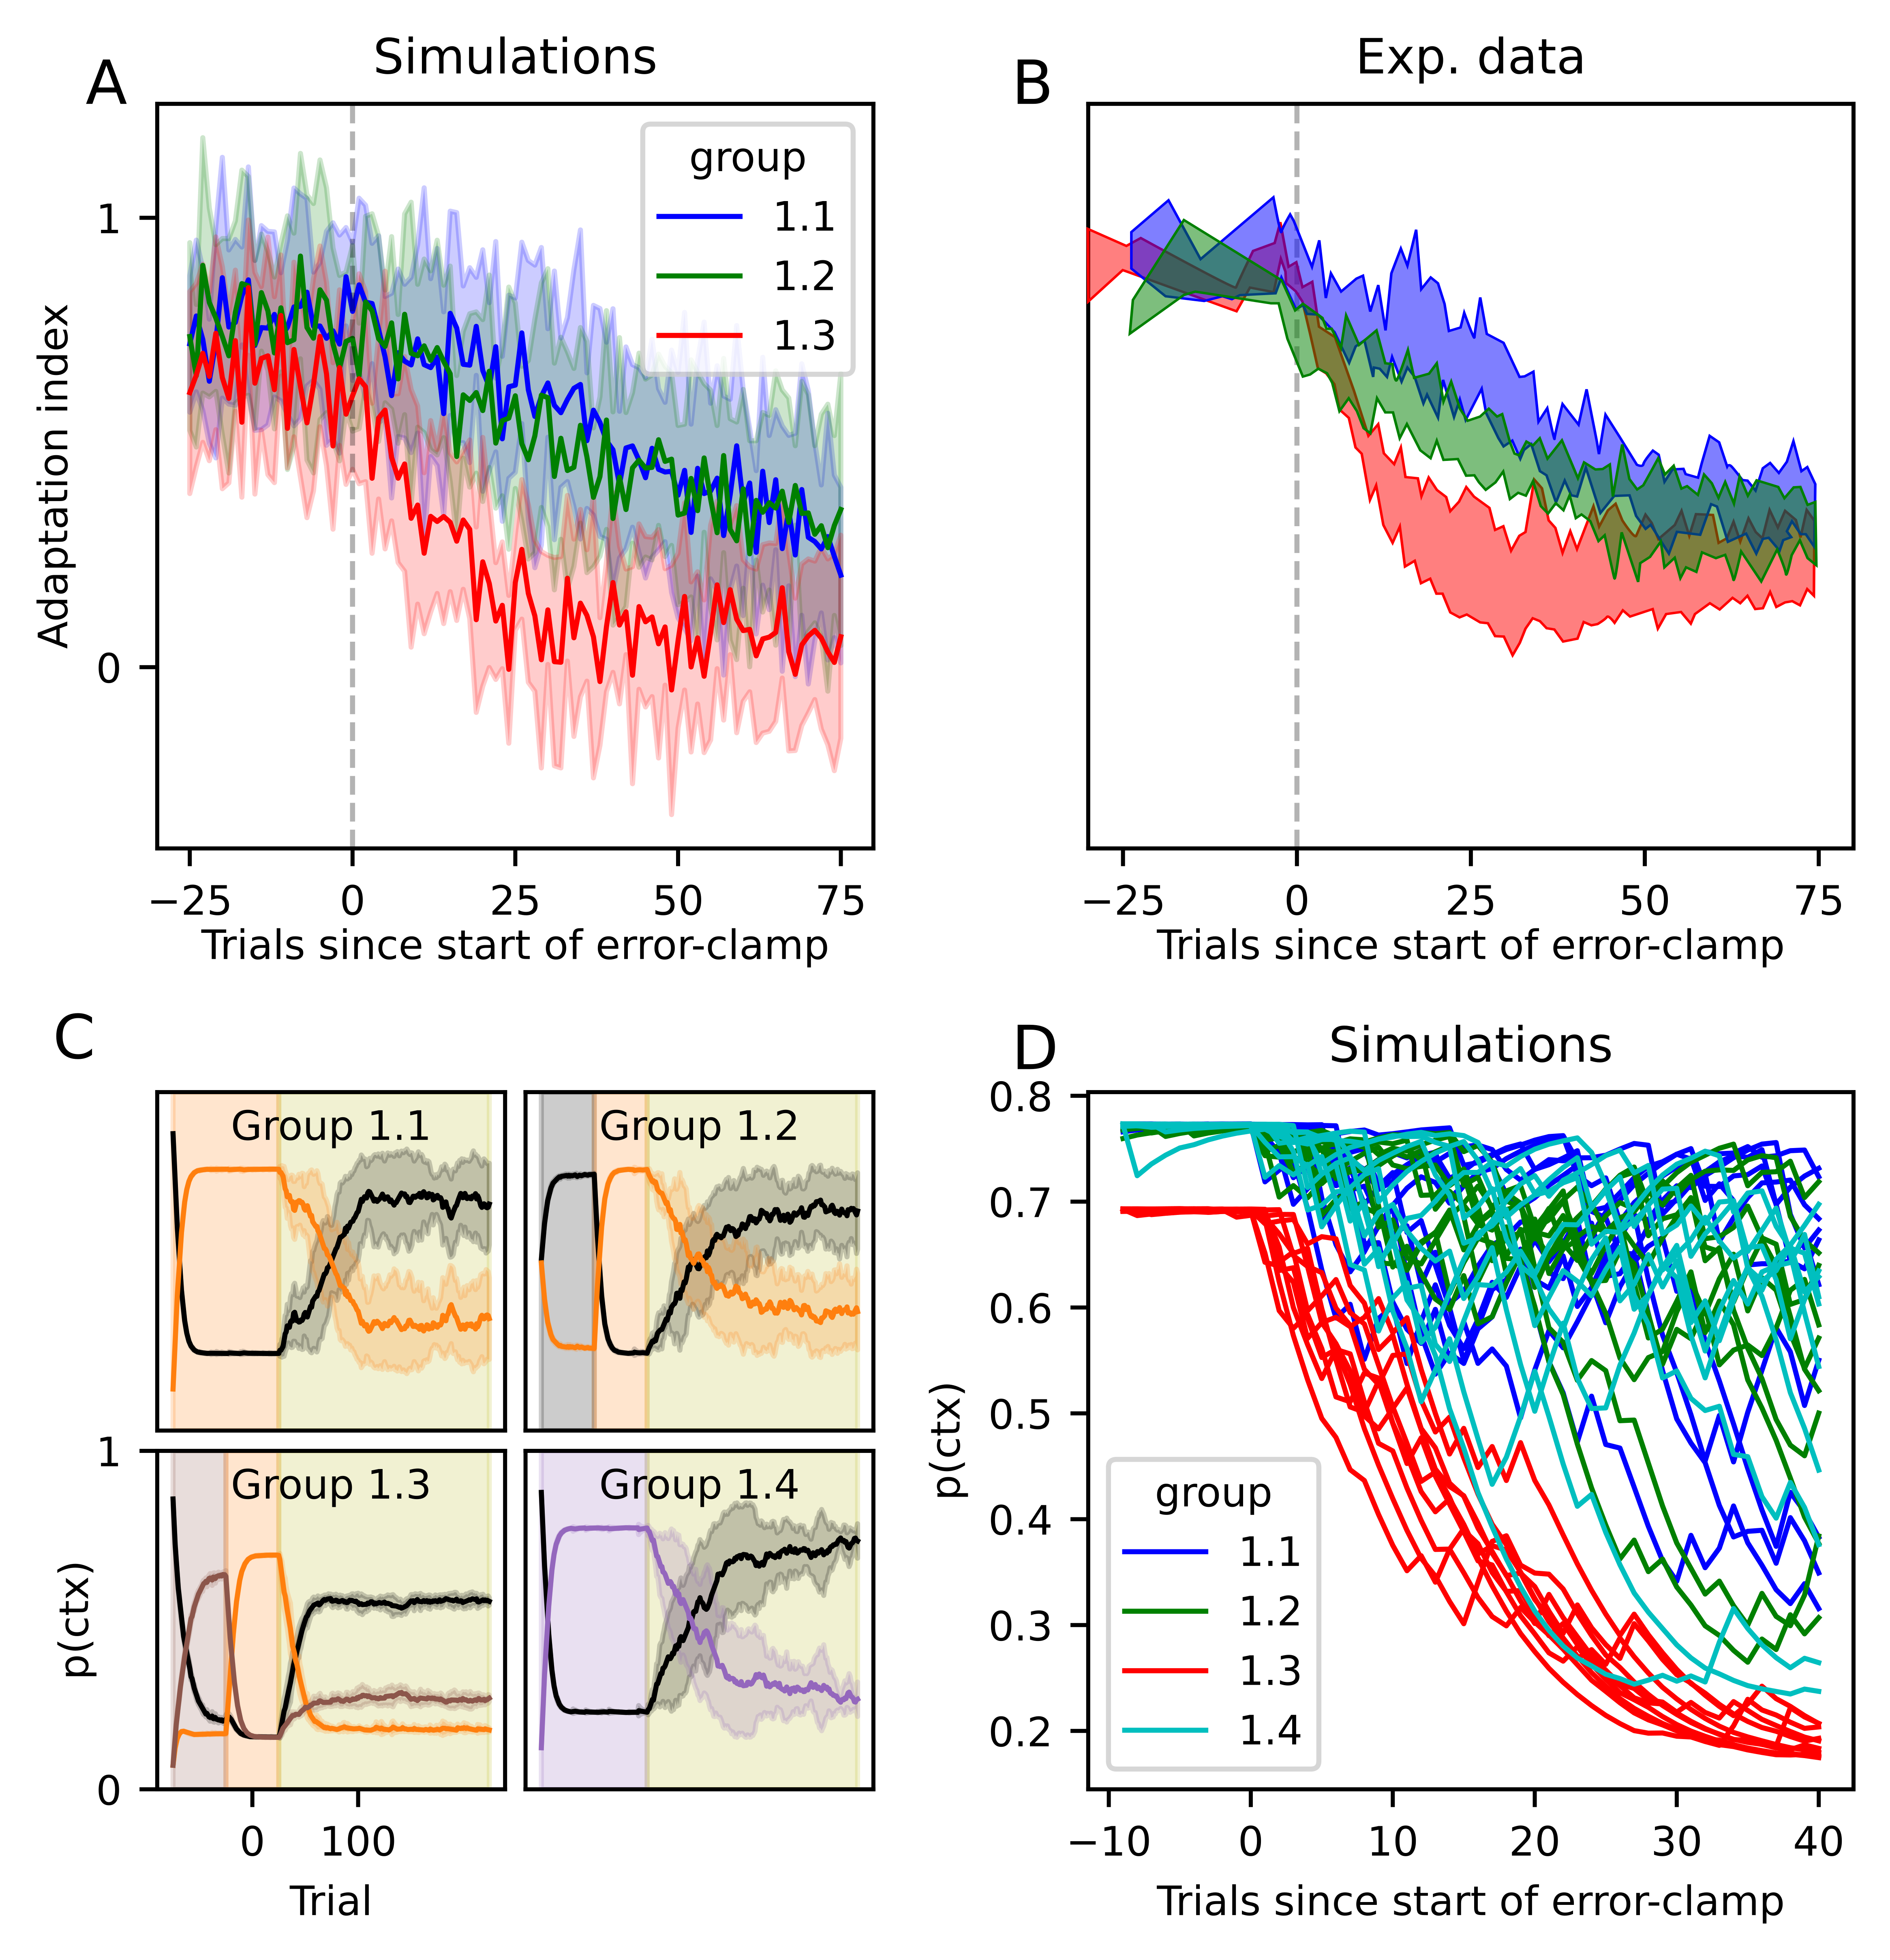
\includegraphics[width=\textwidth]{./figures/figure_4.png}
\caption{Adaptation during error clamp trials. (A) On top, adaptation index shown by the agent belonging to group 1.1 at every trial, i.e. how much the agent adapted to the force that was present, where 1 is optimal adaptation. On bottom, inference over the current context, where contexts are color coded: black for baseline, orange for counter-clockwise force, purple for clockwise force and brown for clockwise force with half strenght. The lines represent the posterior probability of each ocontext at every trial, while the background color represents the real context. An olive-colored background represents error-clamp trials. (B) Same as A, for group 1.2. (C) Same as A, for group 1.3. (D) Same as A, for group 1.4. (E) Simulated data for all groups (same color coding as A-D), only during error-clamp trials. Perceptual noise (i.e. how well the agent can estimate the position of its own hand) was lowered to increase the clarity of the plotted lines; however, increasing it does not change the results. (F) Data adapted from Vaswani et al. 2013, figure 2C, depicting the data equivalent to (E).}
\label{fig:vaswani-2013}
\end{figure}

As can be seen in FIGURE XXX, our model also reproduces the lag before the tapering off in the E block starts. In the model, this lag is due to a period in which context inference has not ``caught on'' to the change of context; during this period, behavior remains consistent with that of the previously-observed block, as can be seen in the experimental data as well. \todo{Simulate the lag? May be worth it}

\section{Discussion}
Discuss that our model does not fully match vaswani in how it all decays. This is because our model does not have a mechanism to create new internal models.

During these error-clamp trials, the natural variability of movements leads to prediction error: during a normal (e.g. A) block, if the participant exerts less force than necessary by mistake, she observes a motor error which, if the adaptation is complete, produces no prediction error. However, in E trials, no error is observed, which leads to a predicted error that is not observed. It is this prediction error that lets the participant know that a transition has occurred. \cite{Vaswani_Decay_2013} performed an additional experiment in which they masked this lack of error by introducing artificial variability on the end position of the hand that mimicked that seen in the participant. Because this eliminated the only source of information regarding a switch of context, participants could no longer infer a switch. Consistent with our model, the authors found that no tapering off occured during the E block. \todo{Moved from Results}

\section{Methods}
\subsection{Model description}
\label{subsection:model-description}
We first describe the general principle behind the model, followed, in the next
subsection, by the full mathematical description of each one of its components.

One of the strenghts of this model is that its general principle does not
depend on the specifics of the experiment to which it is applied. However, for
clarity, we will connect the different parts of the model to different
experiments.

This model is a Bayesian alternative to the N-state learners from
\citep[e.g.][]{Lee_Dual_2009}. In this model, there are no explicit different
timescales and multiple states; instead, the model relies on Bayesian learning
for motor adaptation, combined with inference over the current context.

Before proceding with the model description, let us introduce nomenclature:
\begin{itemize}
\item $t$: Time at the moment an observation is made, before inference is done.
\item $\theta_t$: Observation. Note that this is assumed to be a noisy
observation of the generalized state (see below) given by $\theta_t = h(z_t)$.
\item $s_t$: Hidden state, e.g. the position of the hand in reaching
experiments. It does not depend on the context.
\item $a_t$: Action taken after observing $\theta_t$ and inferring the context.
\item $c_t$: Context inferred after observing $\theta_t$.
\item $\omega_t$: Contextual information. This term includes, e.g. visual cues,
proprioceptive feedback, performance feedback.
\item $z_t$: Generalized state, $z_t = \{s_t, c_t, \omega_t\}$. Observed noisily
as $\theta_t$.
\end{itemize}

Context inference can work through context-specific (possibly unreliable) cues,
or through the dynamics of the system (e.g. expected outputs of motor
commands), using prediction error as the force behind inference. In this case,
the generative model can is written as follows:
\[
p(z_t, z_{t-1}, a_{t-1}, \theta_t, \theta_{t-1}) = p(\theta_t | z_t)p(z_t|\theta_{t-1}, a_{t-1})
\]
and inferring the current (hidden) generalized state is done with Bayes' theorem:
\[
  q(z_t | \theta_t, \theta_{t-1}, a_{t-1}) \propto p(\theta_t | z_t)p(z_t|\theta_{t-1}, a_{t-1})
\]
  
Additionally, after having inferred the current state, motor adaptation is given by
\[
q(\gamma | z_t, z_{t-1}, a_{t-1}) \propto p(z_t | z_{t-1}, a_{t-1}, \gamma)p(z_{t-1})p(\gamma)
\]

where $\gamma$ are the parameters of the internal model for the dynamics,
i.e. the function $f: (z_t, a_t) \rightarrow z_{t+1}$, which determines the beliefs of
the agent regarding how the system evolves after having taken action $a_t$.

Having inferred the generalized state (including context), a decision is made
sampling from a distribution:
\begin{equation}
p(a_t | z_t, \beta) = \displaystyle\sum_{m \in M}q(C_t)p(a_t | z_t, \beta, m)
\end{equation}
where $M$ is the set of all relevant forward models (see below), and
$p(a_t | ... m)$ is the probability distribution over actions prescribed by the
forward model $m$.

In the following sections, we present a specific mathematical implementation
of the principles outlined above. This is the implementation used throughout the
simulations in the main text.

\subsubsection{Mathematical implementation}
The generalized state is given by:
\begin{equation}
z_t = \{x, \theta_t, \gamma_t, \omega_t\}
\end{equation}
where $x$ is, e.g. in a reaching task, the current position of the hand in
Cartesian coordinates, where the origin is the starting point. We assume that
motor commands are issued every $\Delta t$ for simplicity. At the beginning of
each time interval, the context is inferred combining the contextual
information and the prediction error of the outcome of the previous motor
command. This yields:
\begin{align}
  q(C_t) &= q(C_t | \omega_t)q(C_t | s_t, s_{t-1}, a_{t-1}) \\ \label{eqn:estimated-context}
  q(C_t | \omega_t) &\propto p(\omega_t | C_t)p(C_t) \\
  q(C_t | x_t, x_{t-1}, a_{t-1}) &\propto p(x_t | C_t, x_{t-1}, a_{t-1})p(x_t)p(x_{t-1})p(C_t)
\end{align}
The terms $p(C_t)$ refer to the prior probability of the context at the
beginning of the trial: at the first trial, this refers to prior beliefs over
which contexts are more common/likely, which we call $p_0(C_t)$. At each
subsequent trial, it incorporates the belief that has so far been accumulated,
given previous trials. Note that certain events, such as the start of a new
block of trials (see main text) can return an agent to a state in which
$p_0(C_t)$ becomes relevant.

We do not directly model hand movements or eye position. Instead, we model
systems in the motor error space: the position $s_t = 0$ represents a trial in
which no motor error occurred. We make use of the fact that in most
experiments, motor adaptation needs to happen in one of two directions
(e.g. clockwise vs. counter-clockwise) to keep the error space
two-dimensional. With this, $s_t > 0$ represents motor error in one direction
(e.g. clockwise) and $s_t < 0$, error in the other direction. We made this
choice because, in this work, we would model different experiments with
different state spaces; but all these experiments have the commonality of
two-dimensional error spaces. In order to model a specific experiment in its
own physical space (e.g. hand positions in a reaching task), only the dynamical
system of \eref{eqn:dynamical-system} would need to be adapted.

We assume that the decision-making agent has an internal forward model that
maps motor commands to outcomes:
\begin{equation}
p(s_{t+1} | s_t, a_t, m) = f_m(s_t, a_t)
\end{equation}
where $a_t$ are motor commands (actions). We further assume that participants
have learned $f_m$ throughout their lives and use it to decide which motor
command to issue. When a perturbation is introduced, to which the participant
must adapt, we assume they learn a new forward model $f_m^{\phi}$, where $\phi$
represents the parameters of the function that participants must learn. For
example, in a saccade task, $\phi$ represents the new gain. Note that $\phi$
depends on the context and participants need to use and update multiple
forward adapted models $f_m^{\phi}$ throughout one experiment.

Given a forward model $f_m$ (or $f_m^\phi$), action selection is done by
building a probability distribution over possible actions $a_t$ based on how
likely they are to produce zero motor error. For example, in saccade
experiments, motor commands are issued based on how likely they are to move the
fovea to the target. These motor commands are issued to counteract intrinsic
sources of error, such as muscle variability \todo{expand this?}, and extrinsic
sources of error, such as the experimental manipulations on saccade gain. Thus,
the expected observed error can be written as:
\begin{equation}
p(\epsilon | a_t) \propto p(\epsilon_{\text{intrinsic}} | a_t) + p(\epsilon_{\text{extrinsic}} | a_t)
\end{equation}
and a motor command can be chosen to maximize the chance of observing zero error:
\begin{equation}
p(a_t) = argmin_{a_t} p(\epsilon | a_t)
\end{equation}

For simplicity, we assume that motor errors are Gaussian, such that:
\begin{equation}
p(\epsilon | a_t) = N(\mu_{\text{extrinsic}}, \sigma_\epsilon)
\end{equation}
where $\sigma_\epsilon$ incorporates both intrinsic and extrinsic sources of
error. The mean of the error is assumed to have no component, as motor
commands, in the absence of external errors, should produce an error centered
at zero [CITATION MISSING].

With this, a forward model will produce a motor command with outcomes centered
at $-\mu_{\text{extrinsic}}$, which counteracts the externally-induced errors.

To complete the action-selection picture, we return to context inference. As
discussed above, action selection is made via a weighted sum of the different
forward models:
\begin{equation}
p(a_t | ...) \propto \displaystyle \sum_{m \in M} q(C_i)p(a_t | m)
\end{equation}
From this distribution, an action is sampled at each trial.

To update the agent's estimates on the parameters of the forward models, we
make use of Bayes' theorem with conjugate priors. This approach has the
advantage of not only greatly simplifying computational calculations, but also
presenting update equations with great intuitive appeal.

In the following equations, we drop the dependence on the context and
observations for notational simplicity:
\begin{equation}
q(\phi | s_{1:t}) \propto p(s_{1:t} | \phi)p(\phi)
\end{equation}
where $s_{1:t}$ are the observed states up until time $t$. The likelihood will
be a Gaussian:
\begin{align}
  p(s_t | \theta) &= N(\mu_x, \sigma_x)  \\
  \mu_x &= \theta_{t-1} + x \\
  \sigma_x &= \xi_0 1
\end{align}
This likelihood is the probability of observing $x$ given the previous estimate
of the parameters of the force field $\phi_{t-1}$, and given the dynamics of
the system (see below).

To update $\phi$, we assumed that for each context, the agent's belief over
the magnitude of the adaptation is given by a normal distribution:
\begin{equation}
p(\phi) = N(\mu_\phi, \sigma_\phi) \label{eqn:data-dist}
\end{equation}
where $\mu_\phi$ and $\sigma_\phi$ are parameters to be estimated at each
trial. Before the experiment begins, the agent will have a prior distribution
over these parameters. A standard Bayesian approach is to choose NormalGamma
priors:
\begin{equation}
p(\mu_\phi, \sigma_\phi) = NG(\mu_0, \nu_0, \alpha_0, \beta_0)
\end{equation}
where $\mu_0, \nu_0, \alpha_0$ and $\beta_0$ are free hyperparameters of the
model. We assume the following hyperparameter values \todo{Justify}:
\begin{align} \mu_f^{(0)} &= (0, -1, 1) \\
  \nu_f^{(0)} &= 0.1 \\
  \alpha_f^{(0)} &= 1 \\
  \beta_f^{(0)} &= 0.5
\end{align}
Note that $\mu_f^{(0)}$ is different for each context and is thus provided as a
vector $(0, -1, 1)$ representing the baseline and two opposing adaptations
(e.g. clockwise and counter-clockwise visuomotor rotations), respectively. For
all other hyperparameters, all contexts have the same value. These values
ensure that the prior over the hyperparameters $(\mu_\phi, \sigma_\phi)$ has the mode
at $(\mu_\phi^{(0)}, 1)$.

The update equations for the magnitud parameters are given by:
\begin{equation}
q(\mu_f, \sigma_f | x_t, x_{t-1}, a_{t-1}) \propto p(x_t |
x_{t-1}, a_{t-1}, C_t)p(\mu_f, \sigma_f) \label{eqn:context-from-x}
\end{equation}
where $p(x_t | x_{t-1}, a_{t-1}, C_t)$ is a Gaussian distribution centered
around $\mu_a$ with standard deviation $\sigma_a$, which is a free parameter of
the model. It is assumed that the standard deviation over outcomes ($\sigma_a$)
is related to that of the parameter $\mu_f$ as follows:
\begin{equation}
\sigma_f = \sigma_a / \nu_f
\end{equation}
which makes $\nu_f$ a parameter to estimate. Each one of the forward models can
be updated at every trial, depending on context inference (see main text). The
updated parameters for any one forward model $i$ are given by:
\begin{align}
  \mu_\phi^{(t)} &= \frac{\nu_\phi^{(t-1)} \mu_\phi^{(t-1)} + q(C_i)s_t}{\nu_\phi^{(t-1)} + q(C_i)} \\
  \nu_\phi^{(t)} &= \nu_\phi^{(t-1)} + q(C_i) \\
  \alpha_\phi^{(t)} &= \alpha_\phi^{(t-1)} + q(C_i) / 2 \\
  \beta_\phi^{(t)} &= \beta_\phi^{(t-1)} + \frac{q(C_i)\nu_\phi^{(t-1)}}{\nu_\phi^{(t-1)} +
                  q(C_i)}\frac{\left(s_t - \mu_\phi^{(t-1)}\right)^2}{2}
\end{align}
where $q(C_i)$ is the posterior probability of context $C_i$ from
\eref{eqn:estimated-context}. Note that when $q(C_i) = 0$, the model $i$ is not
updated.

The effect of the hyperparameters of the priors are worth a note or two, as
they are complex.

Naturally, $\mu$ affects the initial estimate of the adaptation, in the same
units as the necessary adaptation. $\nu$ encodes how stable this hyperprior is:
higher values (e.g. 10000) all but guarantee that the hypermean will not move
in the face of evidence; In principle, enough evidence should still move it,
but that won't happen during an experiment. Smaller values (e.g. 1 / force\_sd,
as is the default on the code) make the hypermean (and thus the mean) follow
evidence more freely. Note that as more observations are accumulated, $\nu$
becames bigger and bigger, solidifying the value of the hypermean.

The hyperparameters $\alpha$ and $\beta$ are a bit more complex. Note that the
mean of a Gamma distribution is $\beta / (\alpha \nu)$; this mean is being used
as the standard deviation of a Gaussian by the rest of the agent (cheating),
which makes it an important measure of uncertainty. While setting the default
hyperparameters, the values used are $\alpha = 0.5 / \sigma_0$ and
$\beta = 0.5$, where $\sigma_0$ is the \textit{a priori} estimate of the
standard deviation of the force exerted by the environment (force\_sds in the
code), which controls the initial learning rate. This makes the initial
standard deviation equal $\sigma_0$, which makes it consistent with the
fixed-force model in its interface. The 0.5 values ensure that uncertainty is
large at the beginning and during the experiment is greatly reduced, but never
to a point where it's ``visually'' too small. Changing this 0.5 would make the
standard deviation change more quickly, making the model more or less precise
in its predictions, independently of the volatility of the mean of the
adaptation (via the hypermean).

The baseline model defaults to different values that make it a lot more
stable. The hyperstd of the mean is set to 10,000, which makes the mean
entirely stable during the duration of the experiment. The values of $\alpha$
and $\beta$ are fixed regardless of $\sigma_0$ such that the standard deviation
is 0.001 (compare that to the size of the adaptations, around 0.0125), and the
hyperparameters of the standar deviation are stable during the experiment.



\section{Discussion}
\begin{enumerate}
\item The effect of pauses?
\end{enumerate}



\bibliography{../../MyLibrary}


\end{document}
